\documentclass{beamer}

\usepackage{Vor2018glærur}


\usetikzlibrary{arrows}

\title{Tölvunarfræði 2}
\subtitle{Vika 12}

\begin{document}

\begin{frame}
	\titlepage
\end{frame}

\section{Dæmi um hagnýtingu}

\begin{frame}{Schulze kosningakerfið}
	\begin{itemize}
		\item Kunnuglegasta kosningakerfið á Íslandi - hver kjósandi hefur eitt atkvæði, regla D'Hondt notuð til að úthluta sætum
		\item Getum notað atkvæðaseðla þar sem kjósendur forgangsraða frambjóðendum til að mynda annars konar kerfi
		\item Skoðum Schulze kosningakerfið, þar sem sterkustu vegir \eng{strongest paths} í stefndu vegnu neti eru reiknaðir til að komast að því hvaða
	\end{itemize}
\end{frame}

\begin{frame}{Framkvæmd Schulze}
	\begin{itemize}
		\item Við getum skipt Schulze-kosningu upp í nokkur skref
		      \begin{enumerate}
			      \item Talning atkvæða. Við teljum atkvæðaseðlana og búum til stefnt net þar sem þyngd örvaleggs frá $a$ til $b$ er fjöldi kjósenda sem kýs $a$ fram yfir $b$
			      \item Útreikningur sterkustu vega. Reiknum út sterkustu vegi \eng{strongest paths} út frá hverjum hnút netsins
			      \item Túlkun á niðurstöðum. Lesum sigurvegara kosninganna út úr styrkjum sterkustu vega
		      \end{enumerate}
		\item Skoðum dæmi (\href{https://en.wikipedia.org/wiki/Schulze_method}{Wikipedia})
	\end{itemize}
\end{frame}

\begin{frame}{Talning atkvæða}
	\begin{columns}
		\column{0.5\textwidth}
		\begin{itemize}
			\item Atkvæðaseðlarnir taka fram forgang
			\item Efsti atkvæðaseðillinn í \texttt{votes.txt} er EBADC, sem þýðir að kjósandinn vill helst frambjóðanda E, svo B, o.s.frv.
			\item Táknum óskir kjósandans með örvalegg, einn kjósandi gefur þyngdina 1
		\end{itemize}
		\column{0.5\textwidth}
		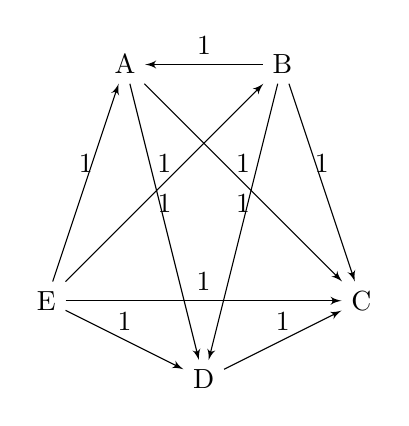
\begin{tikzpicture}
			\tikzset{edge/.style = {->,> = latex'}}
			\node (a) at (2, 5) {A};
			\node (b) at (4, 5) {B};
			\node (c) at (5, 2) {C};
			\node (d) at (3, 1) {D};
			\node (e) at (1, 2) {E};

			\draw[edge] (e) to node[above]{1} (b);
			\draw[edge] (e) to node[above]{1} (a);
			\draw[edge] (e) to node[above]{1} (d);
			\draw[edge] (e) to node[above]{1} (c);
			\draw[edge] (b) to node[above]{1} (a);
			\draw[edge] (b) to node[above]{1} (d);
			\draw[edge] (b) to node[above]{1} (c);
			\draw[edge] (a) to node[above]{1} (d);
			\draw[edge] (a) to node[above]{1} (c);
			\draw[edge] (d) to node[above]{1} (c);
		\end{tikzpicture}
	\end{columns}
\end{frame}

\begin{frame}{Talning atkvæða}
	\begin{columns}
		\column{0.5\textwidth}
		\begin{itemize}
			\item Öll atkvæðin í \texttt{votes.txt} gefa eftirfarandi net. Hér vildu t.d. 25 kjósendur B fram yfir A.

			\item Færri kjósendur vildu A fram yfir B en öfugt, slíkir leggir eru ekki sýndir til að gera myndina greinilegri.
		\end{itemize}
		\column{0.5\textwidth}
		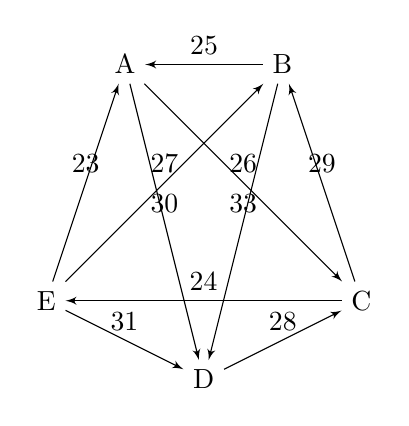
\begin{tikzpicture}
			\tikzset{edge/.style = {->,> = latex'}}
			\node (a) at (2, 5) {A};
			\node (b) at (4, 5) {B};
			\node (c) at (5, 2) {C};
			\node (d) at (3, 1) {D};
			\node (e) at (1, 2) {E};

			\draw[edge] (a) to node[above]{30} (d);
			\draw[edge] (a) to node[above]{26} (c);
			\draw[edge] (b) to node[above]{25} (a);
			\draw[edge] (b) to node[above]{33} (d);
			\draw[edge] (c) to node[above]{29} (b);
			\draw[edge] (c) to node[above]{24} (e);
			\draw[edge] (d) to node[above]{28} (c);
			\draw[edge] (e) to node[above]{31} (d);
			\draw[edge] (e) to node[above]{23} (a);
			\draw[edge] (e) to node[above]{27} (b);
		\end{tikzpicture}
	\end{columns}
\end{frame}

\begin{frame}{Útreikningar sterkustu vega}
	\begin{columns}
		\begin{column}{0.5\textwidth}
			\begin{itemize}
				\item Reiknirit Schulze notar það viðmið að sterkasti vegur í gegnum netið tákni sterkasta frambjóðandann
				\item Styrkur vegs er þyngd léttasta leggs hans
				\item Þurfum að reikna sterkustu vegi út frá hverjum hnút, til þess er hægt að nota tilbrigði við Floyd-Warshall reikniritið
				\item Floyd-Warshall vinnur á grennslafylkjum
			\end{itemize}
		\end{column}
		\begin{column}{0.5\textwidth}
			\[ d =
				\begin{bmatrix}
					-  & 20 & 26 & 30 & 22 \\
					25 & -  & 16 & 33 & 18 \\
					19 & 29 & -  & 17 & 24 \\
					15 & 12 & 28 & -  & 14 \\
					23 & 27 & 21 & 31 & -  \\
				\end{bmatrix}
			\]
			Sama net og á fyrri glæru, $d_{ij}$ er þyngd leggsins frá $i$ til $j$
		\end{column}
	\end{columns}
\end{frame}

\begin{frame}[fragile]{Floyd-Warshall afbrigði}
	Klassískt Floyd-Warshall (sjá t.d. \texttt{FloydWarshall.java} í algs4) finnur léttustu vegi út frá öllum hnútum. Við notum afbrigði sem finnur sterkustu vegi.
	\javafile[firstline=24, lastline=31, gobble=8, fontsize=\scriptsize, label=Schulze.java]{Code/w12/Schulze.java}
	$p_{ij}$ er styrkur sterkasta vegs frá i til j.
\end{frame}

\begin{frame}{Túlkun}
	\begin{columns}
		\begin{column}{0.5\textwidth}
			\begin{itemize}
				\item Lesum sterkustu vegina úr fylkinu $p$
				\item Hér er E (lína 5) sterkari frambjóðandi en allir hinir, svo E er sigurvegari kosninganna
				\item A (lína 1) er sterkari en allir nema E, svo A er í öðru sæti
				\item E > A > C > B > D
			\end{itemize}
		\end{column}
		\begin{column}{0.5\textwidth}
			\[ 
				p =
				\begin{bmatrix}
					-  & \mathbf{28} & \mathbf{28} & \mathbf{30} & 24 \\
					25 & -  & 28 & \mathbf{33} & 24 \\
					25 & \mathbf{29} & -  & \mathbf{29} & 24 \\
					25 & 28 & 28 & -  & 24 \\
					\mathbf{25} & \mathbf{28} & \mathbf{28} & \mathbf{28} & -  \\
				\end{bmatrix}
			\]
			$p_{ij}$ er styrkur sterkasta vegs frá $i$ til $j$
		\end{column}
	\end{columns}
\end{frame}

\begin{frame}{Næst}

\end{frame}

\end{document}
